\documentclass[a4paper,12pt]{article}
\usepackage[pdftex]{graphicx}
\usepackage[table]{xcolor} % Defines colors (incl. gray) and supports colored tables
\usepackage[hidelinks]{hyperref}
\usepackage{anysize}
\usepackage[utf8]{inputenc}
\usepackage[T1]{fontenc}
\usepackage[portuguese,brazil]{babel}
\usepackage{fancyhdr}
\usepackage{natbib}
\usepackage{amssymb}
\usepackage{amsmath}
\usepackage{subfig} % Figuras lado a lado.
\captionsetup[subfloat]{%
    position=bottom,
    justification=centering
}
\usepackage[scaled]{helvet} % Fonte semelhante à Arial (Helvetica)
\renewcommand{\familydefault}{\sfdefault} % Define fonte padrão como sans-serif
\usepackage{tabularx} % tabelas mais flexíveis
\usepackage{titlesec} % possibilita alterar o formato das seções
\usepackage{parskip} % controle de espaçamento de parágrafos
\usepackage{caption} %Possibilita editar captions.
\usepackage{float}
\usepackage{fontawesome}

\captionsetup{%
    %format=hang,
    justification=raggedright,
    singlelinecheck=false,
    figureposition=top,
    font=small
    }

%%%%%%%%%%%%%% Formatação dos estilos das seções
\titleformat{\section}
 {\normalfont\Large\bfseries}{\thesection.}{0.5em}{}[{\titlerule[0.6pt]}]

%%%%%%%%%%%%% Tabela
\captionsetup[table]{name=Quadro} %Altera o nome de Tabela para Quadro.


%%%%%%%%%%%%% Apelidos para bibliografias
\newcommand{\mnras}{Mon. Not. R. Astron. Soc.}
\newcommand{\aap}{Astronomy $\&$ Astrophysics}
\newcommand{\apjs}{ApJS}
\newcommand{\apj}{Astrophys. J.}
\newcommand{\apjl}{Astrophys. J. Letters}
\newcommand{\aj}{Astron. J.}
\newcommand{\pasa}{PASA}
\newcommand{\nat}{Nature}
\newcommand{\natastron}{Nature Astronomy}

%%%%%%%%%%%%%%%% Espaçamento entre linhas
\renewcommand{\baselinestretch}{1.5} % Espaçamento de 1.5 entre linhas
\setlength{\parskip}{10pt} % espaço entre parágrafos (uma linha em branco).

%%%%%%%%%%%%%% Margens
%\marginsize{left}{right}{top}{bottom}
\marginsize{30mm}{20mm}{30mm}{20mm}

\pagestyle{fancy}
\fancyhf{} % clear all fields
\setlength{\headheight}{45pt} % Avoid fancyhdr warning (adjust if needed)
\addtolength{\topmargin}{-50pt} % Compensate for increased header height
\fancyhead[R]{
	\textcolor{gray}{\small Universidade Federal do Espírito Santo}\\ 
	\textcolor{gray}{\small Programa Institucional de Iniciação Científica} \\
	\textcolor{gray}{\small Relatório Parcial de Pesquisa}\\
	\textcolor{red}{\small Área do Conhecimento (CNPq)}
}
\rfoot{\thepage}
\renewcommand{\headrulewidth}{0pt}

%%%%%%%%%%%%%%%%%%%%%%%%%%%%
%%%%%%%%%%%% Begin Document
\begin{document}

\begin{tabularx}{\textwidth}{|>{\columncolor[gray]{0.9}} l|X|}
\hline
{\bf Edital:} & \textbf{Edital Piic 20-- / 20--  } \\
\hline
{\bf Área do Conhecimento (CNPq):} &   \\
\hline
{\bf Subárea do Conhecimento (CNPq):} &  \\
\hline
{\bf Título do Projeto:}&  \\
\hline
{\bf Título do Subprojeto:} & \\
\hline
{\bf Orientador(a):} & \\
\hline
{\bf Estudante:} & \\
\hline
\end{tabularx}

\begin{tabularx}{\textwidth}{|>{\columncolor[gray]{0.9}}  p{0.418\textwidth}|X|}
\hline
{\bf Estudante apresenta alguma  necessidade de acessibilidade?} & ( )Sim / ( ) Não \\
\hline
{\bf Se sim, informar o recurso ou  suporte de acessibilidade que necessita.} & \\
\hline
\end{tabularx}

\vspace{.5cm}

% Requires: \usepackage{xcolor}

{\color{red}
\noindent{\bfseries Orientações Gerais (remover na versão final)}

\begin{itemize}
  \item Este relatório deve ser elaborado pelo(a) estudante sob supervisão do(a) orientador(a).
  \item O relatório deve ser enviado pelo(a) orientador(a) via Sistema Acadêmico de Pesquisa (SAPPG), conforme as datas do edital.
  \item O atraso no envio pode resultar na suspensão da bolsa e em restrições em edições futuras.
  \item O relatório deve conter as seções: \textbf{Introdução; Materiais e Métodos; Resultados e Discussão; Atividades Realizadas e Metas Futuras; Referências}.
  \item Formatação mínima obrigatória:
    \begin{itemize}
      \item Tamanho A4; margens: 3 cm (superior e esquerda) e 2 cm (inferior e direita)
      \item Fonte \textbf{Arial}, corpo \textbf{12} no texto e \textbf{14} nos títulos
      \item Espaçamento 1,5 entre linhas
      \item Alinhamento justificado
      \item Sem recuo na primeira linha dos parágrafos
      \item Cabeçalho em Arial 10
      \item Inserir, na \textbf{quarta linha do cabeçalho, a área do conhecimento conforme classificação do CNPq}
    \end{itemize}
    \item O documento deve ser exportado em \textbf{PDF}.
\end{itemize}
}

%%%%%%%%%%%%%%%%%%%%%%%%%%%%%
\section{Introdução}
A linguagem utilizada ao longo do trabalho deve ser, sempre que possível, técnica e impessoal, uma vez que se trata de um trabalho acadêmico. Deve-se evitar o uso de gírias e de termos de linguagem coloquial, bem como o uso das primeiras pessoas do singular e do plural (fiz ou fizemos...; obtive ou obtivemos...), e priorizar a estrutura passiva (fez-se...; foram obtidos...). O conteúdo de cada seção deve estar de acordo com as recomendações descritas neste modelo. Na Introdução, o autor deve apresentar, de forma concisa, uma contextualização do tema de sua pesquisa, mostrando sua relevância, justificando o tema escolhido, e descrevendo claramente a sua pergunta ou seu problema de pesquisa. Deve-se também ressaltar a ligação do Subprojeto de Iniciação Científica com o Projeto de Pesquisa ao qual está vinculado. Esta seção deve conter, \textbf{no máximo, 30 linhas.}

%%%%%%%%%%%%%%%%%%%%%%%%%%%%%
\section{Materiais e Métodos}
Nesta seção devem ser descritos, de maneira sucinta, \textbf{em até 30 linhas}, o detalhamento da metodologia utilizada no decorrer da pesquisa executada pelo discente no primeiro semestre de vinculação ao Piic/Ufes, bem como os procedimentos de trabalho adotados, os materiais que foram utilizados, o tratamento da informação realizado e o procedimento estatístico aplicado, se for o caso. 

%%%%%%%%%%%%%%%%%%%%%%%%%%%%%
\section{Resultados e Discussão}
Esta seção deve explicitar, \textbf{em até 30 linhas}, os principais resultados obtidos no decorrer da pesquisa executada pelo discente no primeiro semestre de vinculação ao Piic/Ufes. Em todo o relatório, ilustrações (figuras, gráficos, fotos, fluxogramas, quadros e etc.) e tabelas podem também ser incluídas e devem ser utilizadas a fim de de organizar os dados, realizar comparações, sintetizar informações e dar suporte às análises. Deve-se destacar que tais ilustrações ou tabelas não são computadas como linhas do texto. As ilustrações e tabelas devem ser inseridas imediatamente após o trecho ao qual fazem referência. Estes elementos devem estar centralizados na página. Na parte inferior, deve constar a indicação da fonte consultada (elemento obrigatório, mesmo que seja “produção do próprio autor”), legenda, notas e/ou outras informações necessárias à compreensão (se houver), como mostra a Figura \ref{fig:exemplo1}. 


\begin{figure}[H]
    \centering
    \caption{(a) Fotografia do modelo de edificação utilizado no experimento e (b) representação esquemática do comportamento do escoamento sobre a edificação. Fonte: [CITAR AQUI].}
    \label{fig:exemplo1}
    \subfloat[]{
        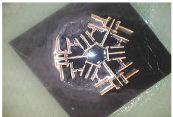
\includegraphics[width=0.48\textwidth]{Picture1.png}
    }
    \hfill
    \subfloat[]{
        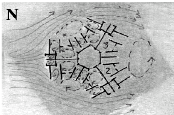
\includegraphics[width=0.48\textwidth]{Picture2.png}
    }
\end{figure}


Para inserir números de figuras, inclua uma etiqueta (\textit{label}) dentro do ambiente de figura (\verb|\label{fig:exemplo1}|) e refira ao mesmo usando \verb|\ref{fig:exemplo1}|. Links são criados automaticamente. O uso de ``fig:'' na etiqueta da figura é prática comum e recomendada, mas qualquer nome de etiqueta funciona.

No caso de figuras e tabelas, sugere-se a inserção de um texto alternativo, que é uma breve descrição textual que permite a pessoas com deficiência visual, que utilizam softwares leitores de tela, compreender o conteúdo visual do relatório.

\textbf{Orientações para a redação do texto alternativo:}

\begin{itemize}
    \item \textbf{Seja objetivo:} Comece pela informação mais importante. Evite expressões como ``Imagem de...'' ou ``Foto de...'', pois o leitor de tela já identifica o elemento como gráfico.
    
    \item \textbf{Hierarquia de dados:} Em gráficos, descreva primeiro o tipo (por exemplo, ``Gráfico de barras''), o título e os valores de maior destaque ou a tendência geral.
    
    \item \textbf{Contexto científico:} Descreva apenas o que é relevante para a pesquisa. Se uma cor no gráfico indica uma variável específica, mencione-a; se for apenas decorativa, não é necessário descrevê-la.
    
    \item \textbf{Tabelas:} Certifique-se de que a descrição resuma a principal conclusão que os dados da tabela apresentam.
\end{itemize}



%%%%%%%%%%%%%%%%%%%%%%%%%%%%%
\section{Atividades Realizadas e Produtos do Projeto}
Ao longo do período de vigência deste projeto de Iniciação Científica, todas as atividades planejadas foram executadas com sucesso, culminando em uma análise robusta e na produção de resultados científicos relevantes. As tarefas executadas podem ser resumidas da seguinte forma:

Primeiramente, foi realizado um aprofundamento teórico sobre os temas de matéria escura, dinâmica galáctica e métodos estatísticos, consolidando a base de conhecimento necessária para a pesquisa. Em paralelo, foram desenvolvidas as habilidades de programação em \texttt{Python}, com foco nas bibliotecas científicas essenciais para a análise de dados astrofísicos.

A etapa seguinte consistiu na familiarização com o catálogo de dados \texttt{SPARC}. Foi desenvolvido um \textit{pipeline} de software para ler, processar e visualizar as curvas de rotação. Inicialmente, foram implementados ajustes de perfis de matéria escura utilizando métodos de otimização baseados em $\chi^2$ e busca em grade, cujos resultados para diversas galáxias foram apresentados na XLVII Reunião Anual da Sociedade Astronômica Brasileira.

Posteriormente, a metodologia foi refinada para uma abordagem de inferência Bayesiana completa, utilizando MCMC. Essa análise mais sofisticada, aplicada a uma amostra de galáxias HSB e LSB, resultou em um trabalho que foi aceito para apresentação em formato de pôster na conferência internacional \textit{Galaxy Memoirs 2025}, realizada em Armação Buzius, Rio de Janeiro. A análise foi executada utilizando os recursos computacionais do cluster \textit{Sci-Com} do Núcleo Capixaba de Computação Científica (NC3), que foi fundamental para a viabilidade do processamento intensivo exigido pelo MCMC.

\begin{table}[H]
\caption{Lista de atividades previstas e realizadas do Subprojeto.}
\begin{tabularx}{\textwidth}{|X|}
\hline
1 -  Programação em Python \& \textit{Wolfram Language}: constante desenvolvimento. \\
\hline
2 - Potencial gravitacional em gravitação Newtoniana para modelagem de galáxias. \\
\hline
3 - Modelos de matéria escura e gravitação.  \\
\hline
4 - Familiarização com o \textit{sample} de dados SPARC.  \\
\hline
5 - Otimização de $\chi^2$. \\
\hline
6 - Determinação de parâmetros de modelos, com regiões de confiança, a partir de análise Bayesiana. \\
\hline
7 - Atividades complementares: Limpeza dos códigos e preparação para publicação no Github; Apresentação em eventos. \\
\hline
8 - Relatório parcial. \\
\hline
9 - Relatório final. \\
\hline
\end{tabularx}
{\small Fonte: Produção do próprio autor.}
\end{table}

\begin{table}[H]
\caption{Cronograma de atividades do Subprojeto, indicando a conclusão das tarefas.}
\begin{tabularx}{\textwidth}{|l|c|c|c|c|c|c|c|c|c|c|c|c|}
\hline
\rowcolor[gray]{.9}
Atividade &  set & out & nov & dez & jan & fev & mar & abr & mai & jun & jul & ago\\
\hline
1 & \faSmileO  & \faSmileO  & \faSmileO  & \faSmileO   & \faSmileO & \faSmileO  & \faSmileO  & \faSmileO  & \faSmileO  & \faSmileO  & \faSmileO  & \faSmileO \\
\hline
2 & \faSmileO & \faSmileO  & \faSmileO  &   &   &   &   &   &   &   &   &  \\
\hline
3 &   & \faSmileO  & \faSmileO  & \faSmileO  & \faSmileO &   &   &   &   &   &   &  \\
\hline
4 &   & \faSmileO  & \faSmileO  & \faSmileO  &   &  &   &  &  &  &   &  \\
\hline
5 &   &   &  \faSmileO &  \faSmileO  & \faSmileO & \faSmileO  & \faSmileO  &   &   &   &   &  \\
\hline
6 &   &   &   &    &   &   & \faSmileO  &  \faSmileO & \faSmileO  & \faSmileO  & \faSmileO  &  \\
\hline
7 &   &   &   &   &   &   &   &  \faSmileO  & \faSmileO  & \faSmileO  & \faSmileO  & \faSmileO \\
\hline
8 &   &   &   &   &   & \faSmileO  &   &   &   &   &   &   \\
\hline
9 &   &   &   &   &   &   &   &   &   &   &   & \faSmileO  \\
\hline
\end{tabularx}
{\small Fonte: Produção do próprio autor.}
\end{table}

%%%%%%%%%%%%%%%%%%%%%%%%%%%%%
\section{Agradecimentos}
Agradeço ao Programa Institucional de Iniciação Científica (PIIC) da Universidade Federal do Espírito Santo (UFES) e ao Conselho Nacional de Desenvolvimento Científico e Tecnológico (CNPq) pela bolsa e pelo fomento a esta pesquisa. Agradeço também ao Núcleo Capixaba de Computação Científica (NC3) por disponibilizar a infraestrutura computacional do cluster \textit{Sci-Com}, cujos recursos foram indispensáveis para a execução das amostragens MCMC.

%%%%%%%%%%%%%%%%%%%%%%%%%%%%%
\section{Atividades Complementares}
Durante a execução deste projeto, os resultados parciais e finais foram divulgados em importantes fóruns científicos. As principais atividades complementares foram:
\begin{itemize}
    \item \textbf{Apresentação de Pôster:} Participação na XLVII Reunião Anual da Sociedade Astronômica Brasileira (SAB), onde foram apresentados os resultados preliminares da análise de galáxias do catálogo SPARC.
    \item \textbf{Apresentação em Conferência Internacional:} Apresentação de um pôster na conferência \textit{Galaxy Memoirs 2025}, detalhando a análise Bayesiana comparativa entre os perfis de matéria escura em galáxias HSB e LSB.
    \item \textbf{Disponibilização de Código:} O código-fonte em \texttt{Python} desenvolvido para a análise das curvas de rotação está sendo preparado e documentado para publicação em um repositório público no \textit{GitHub}, em alinhamento com as práticas de ciência aberta.
\end{itemize}

%%%%%%%%%%%%%%%%%%%%%%%%%%%%%
\section*{Referências Bibliográficas}
\flushleft{BINNEY, James; TREMAINE, Scott. \textbf{Galactic dynamics}. Princeton university press, 2011.}

\flushleft{BOSMA, A. The distribution and kinematics of neutral hydrogen in spiral galaxies of various morphological types. 1978. \textbf{Thesis (PhD)}. University of Groningen, 1978.}

\flushleft{BURKERT, Andreas. The structure of dark matter halos in dwarf galaxies. \textbf{The Astrophysical Journal}, v. 447, n. 1, p. L25, 1995.}

\flushleft{DE BLOK, W. J. G. The Core‐Cusp Problem. \textbf{Advances in Astronomy}, v. 2010, n. 1, p. 789293, 2010.}

\flushleft{DEL POPOLO, A. \textit{et al}. A unified solution to the small scale problems of the $\Lambda$CDM model. \textbf{Journal of Cosmology and Astroparticle Physics}, v. 2014, n. 04, p. 021, 2014.}

\flushleft{HERNÁNDEZ-ARBOLEDA, Alejandro; RODRIGUES, Davi C. Rotação de galáxias e matéria escura. \textbf{Cadernos de Astronomia}, v. 2, n. 1, p. 6-33, 2021.}

\flushleft{KEETON, Charles. \textbf{Principles of astrophysics}. New York: Springer, 2014.}

\flushleft{LI, Pengfei \textit{et al}. Fitting the radial acceleration relation to individual SPARC galaxies. \textbf{Astronomy \& Astrophysics}, v. 615, p. A3, 2018.}

\flushleft{LELLI, Federico; MCGAUGH, Stacy S.; SCHOMBERT, James M. SPARC: Mass models for 175 disk galaxies with Spitzer photometry and accurate rotation curves. \textbf{The Astronomical Journal}, v. 152, n. 6, p. 157, 2016.}

\flushleft{NAVARRO, Julio F.; FRENK, Carlos S.; WHITE, Simon DM. A universal density profile from hierarchical clustering. \textbf{The Astrophysical Journal}, v. 490, n. 2, p. 493, 1997.}

\flushleft{RODRIGUES, Davi C. \textit{et al}. Evidence against cuspy dark matter haloes in large galaxies. \textbf{Monthly Notices of the Royal Astronomical Society}, v. 470, n. 2, p. 2410-2426, 2017.}

\flushleft{RUBIN, V. C.; FORD, W. K.; THONNARD, N. Extended rotation curves of high-luminosity spiral galaxies. IV - Systematic dynamic properties, SA to SC. \textbf{The Astrophysical Journal}, v. 225, p. L107-L111, 1978.7.}

\flushleft{WALTER, Fabian \textit{et al}. THINGS: The H i nearby galaxy survey. \textbf{The Astronomical Journal}, v. 136, n. 6, p. 2563, 2008.}

\flushleft{ZWICKY, F. The redshift of extragalactic nebulae. \textbf{Helvetica Physica Acta}, v. 6, p. 110-127, 1933.}

\flushleft{ZWICKY, F. On the masses of nebulae and of clusters of nebulae. \textbf{The Astrophysical Journal}, v. 86, p. 217, 1937.}

\end{document}